%%%%%%%%%%%%%%%%%%%%%%%%%%%%%%%%%%%%%%%%%
% The Legrand Orange Book
% LaTeX Template
% Version 2.1.1 (14/2/16)
%
% This template has been downloaded from:
% http://www.LaTeXTemplates.com
% https://pt.overleaf.com/latex/templates/the-legrand-orange-book-template-english/jtctyfmnpppc
%
% Original author:
% Mathias Legrand (legrand.mathias@gmail.com) with modifications by:
% Vel (vel@latextemplates.com)
%
%  License:
%  CC BY-NC-SA 3.0 (http://creativecommons.org/licenses/by-nc-sa/3.0/)
%
% Compiling this template:
% This template uses biber for its bibliography and makeindex for its index.
% When you first open the template, compile it from the command line with the 
% commands below to make sure your LaTeX distribution is configured correctly:
%
% 1) pdflatex main
% 2) makeindex main.idx -s StyleInd.ist
% 3) biber main
% 4) pdflatex main x 2
%
% After this, when you wish to update the bibliography/index use the appropriate
% command above and make sure to compile with pdflatex several times 
% afterwards to propagate your changes to the document.
%
% This template also uses a number of packages which may need to be
% updated to the newest versions for the template to compile. It is strongly
% recommended you update your LaTeX distribution if you have any
% compilation errors.
%
% Important note:
% Chapter heading images should have a 2:1 width:height ratio,
% e.g. 920px width and 460px height.
%
%%%%%%%%%%%%%%%%%%%%%%%%%%%%%%%%%%%%%%%%%

%----------------------------------------------------------------------------------------
%	 PACKAGES AND OTHER DOCUMENT CONFIGURATIONS
%----------------------------------------------------------------------------------------

\documentclass[11pt,fleqn]{book} % Default font size and left-justified equations

\usepackage{ccicons}

\newcommand{\infocaio}[2]{\textbf{Autor:} Caio C\'{e}sar C. Ortega \\ \textbf{Biografia:} aluno da Universidade Federal do ABC, cursa os bacharelados em Ci\^{e}ncias e Humanidades e em Planejamento Territorial. Morador da Zona Leste da capital. Possui cerca de dez anos de experi\^{e}ncia profissional em \textit{call} e \textit{contact center}, principalmente nas \'{a}reas de atendimento, planejamento e MIS. Ajudou a idealizar e iniciar o COMMU em 2014 \\ \textbf{Originalmente publicado em:} {#1} \\ \textbf{Endere\c{c}o do original:} \url{{#2}}}

%----------------------------------------------------------------------------------------

\input{structure} % Insert the commands.tex file which contains the majority of the structure behind the template

\begin{document}

%----------------------------------------------------------------------------------------
%	 TITLE PAGE
%----------------------------------------------------------------------------------------

\begingroup
\thispagestyle{empty}
\begin{tikzpicture}[remember picture,overlay]
\coordinate [below=12cm] (midpoint) at (current page.north);
\node at (current page.north west)
{\begin{tikzpicture}[remember picture,overlay]
\node[anchor=north west,inner sep=0pt] at (0,0) {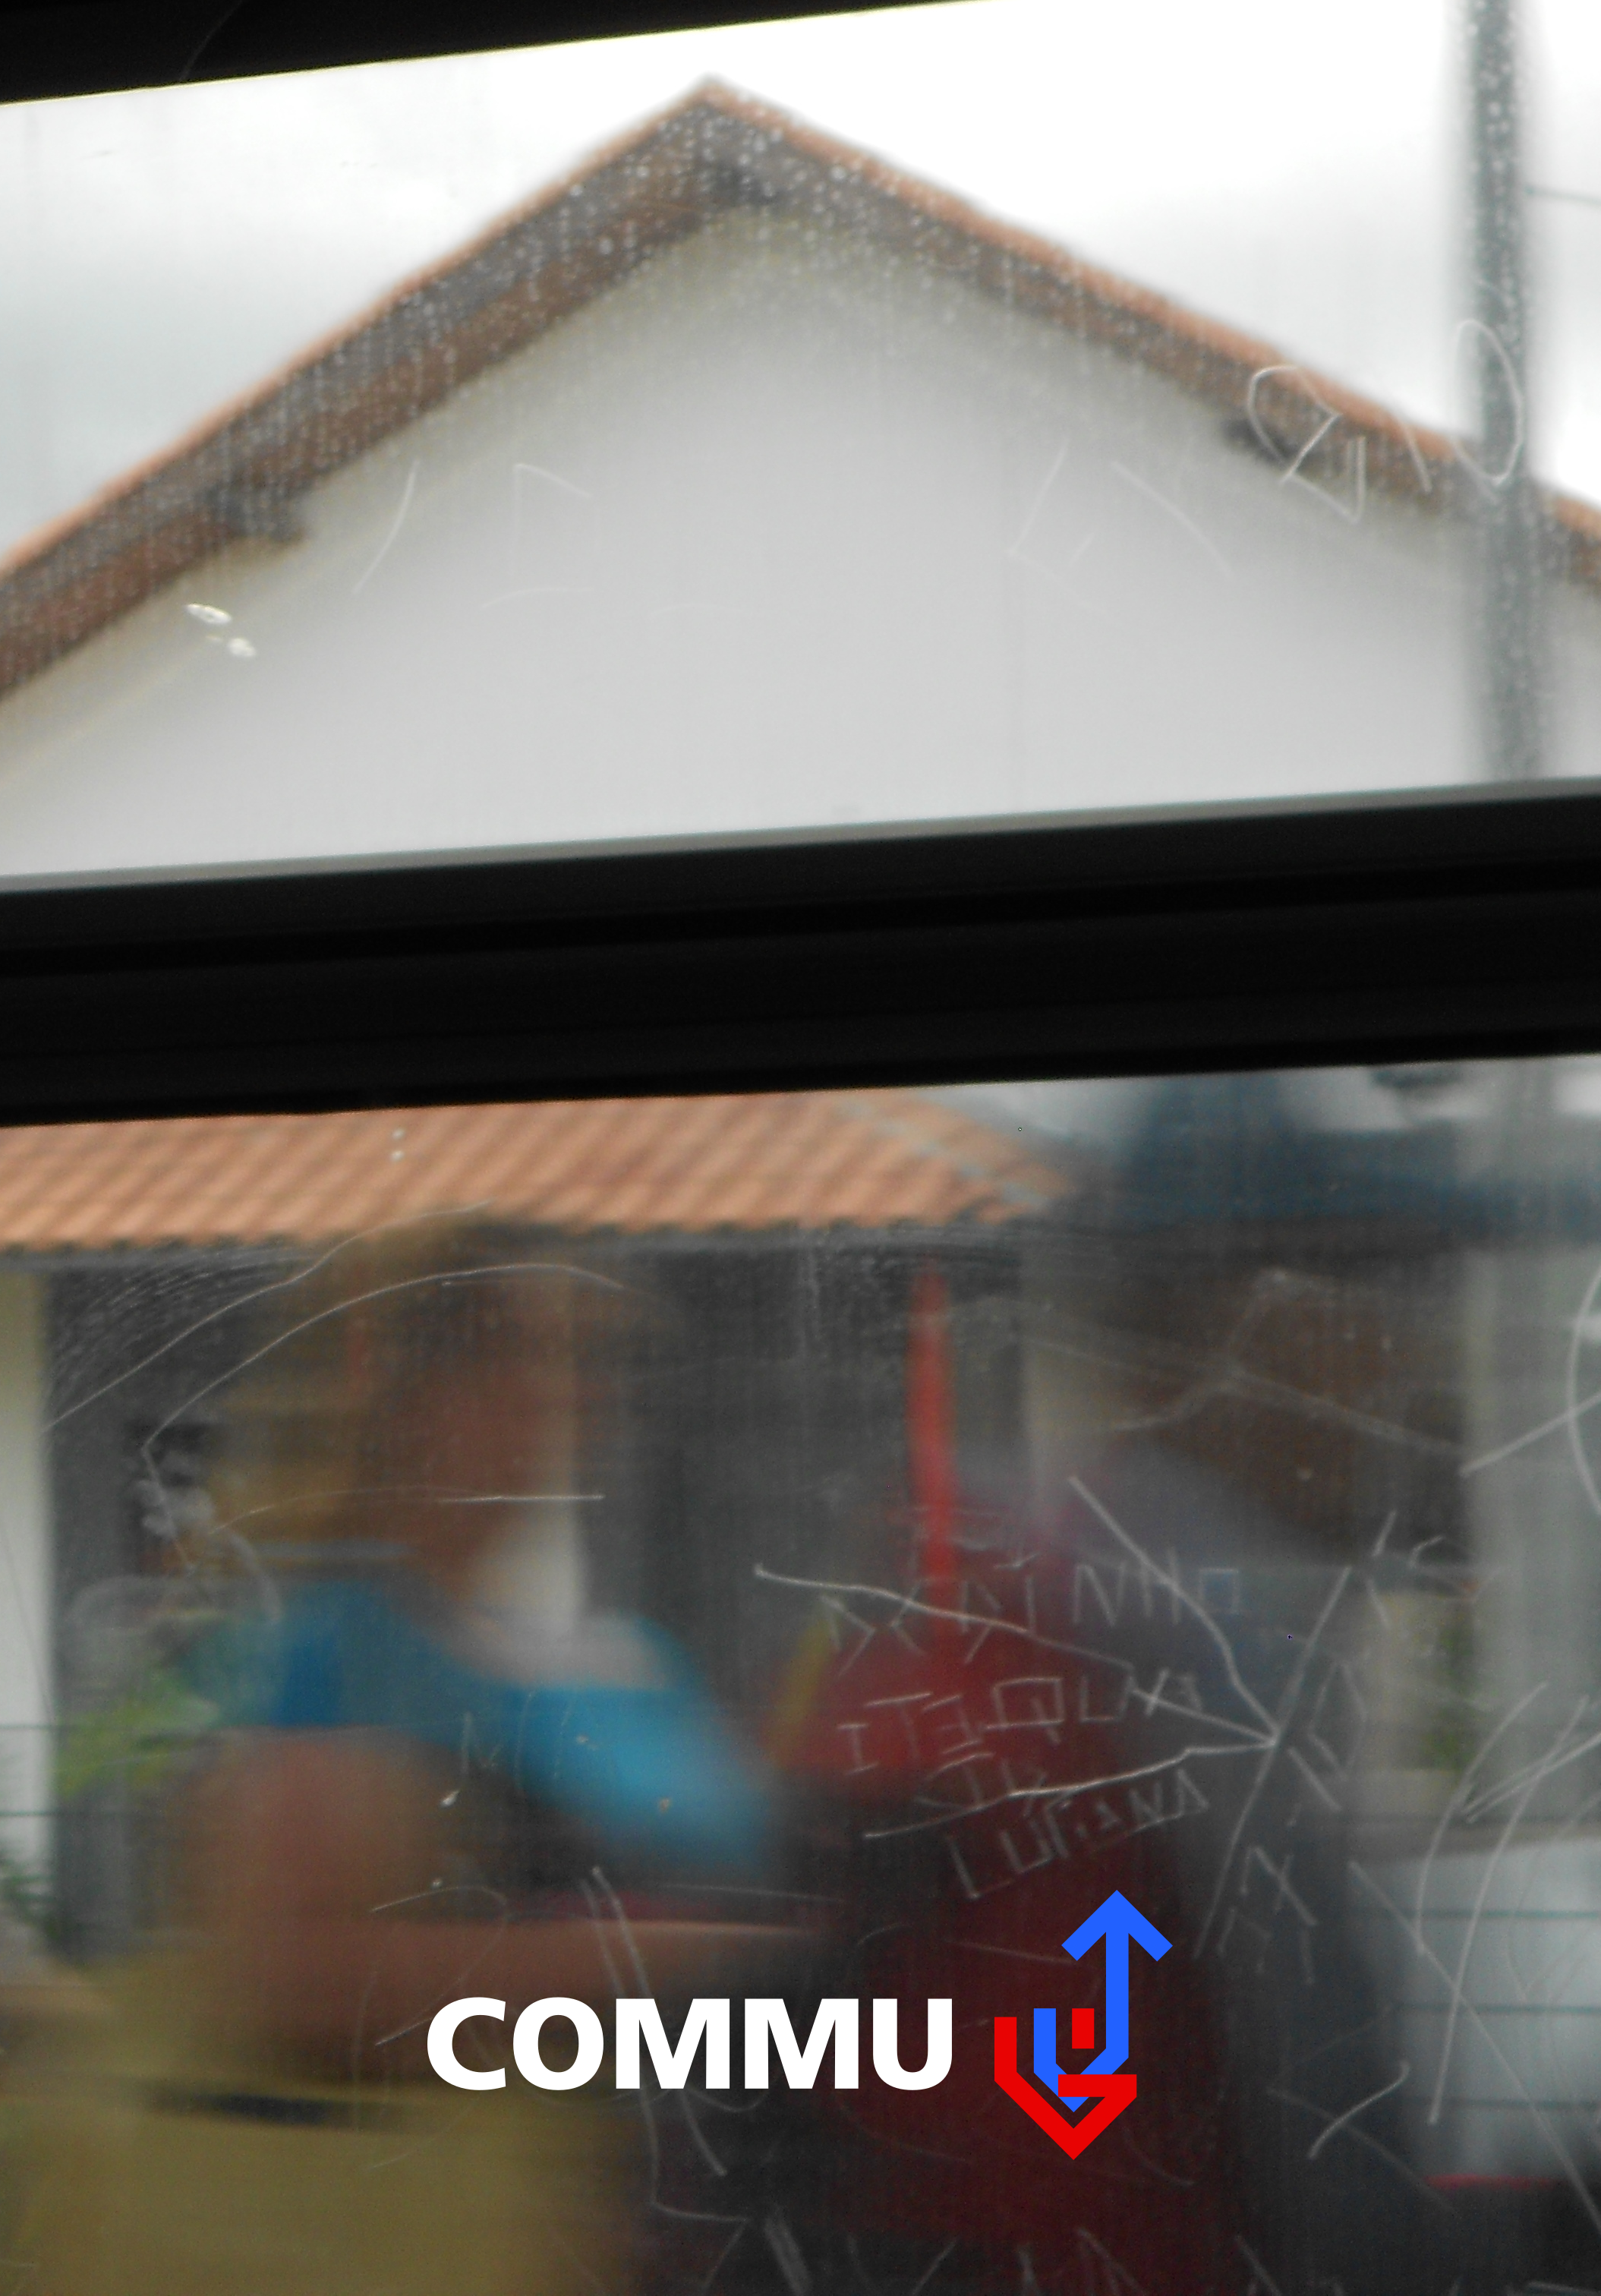
\includegraphics[width=\paperwidth]{2016-10-21_mdc_partida_l11}}; % Background image
\draw[anchor=north] (midpoint) node [fill=black!90!white,fill opacity=0.6,text opacity=1,inner sep=1cm]{\Huge\centering\bfseries\sffamily\parbox[c][][t]{\paperwidth}{\centering \textcolor{white}{Querem privatizar a CPTM. E agora?} \\[15pt] % Book title
{\Large \textcolor{white}{Um arsenal para discussão de problemas e parcerias público-privadas}}\\[20pt] % Subtitle
{\huge \textcolor{white}{Coletivo Metropolitano de Mobilidade Urbana}}}}; % Author name
\end{tikzpicture}};
\end{tikzpicture}
\vfill
\endgroup

%----------------------------------------------------------------------------------------
%	 COPYRIGHT PAGE
%----------------------------------------------------------------------------------------

\newpage
~\vfill
\thispagestyle{empty}

\noindent Alguns direitos reservados ao Coletivo Metropolitano de Mobilidade Urbana, 2019 \\ % Informações de direitos

\noindent \textsc{Publicação independente}\\ % Publicador

\noindent \textsc{medium.com/@commu}\\ %  URL

\vspace{2cm}

\noindent {\Huge \ccbync} \\

\noindent Licenciado sob a \textbf{Licença Creative Commons Atribuição-NãoComercial 3.0-NãoAdaptada} (doravante denominada ``LICENÇA''), regida pelos termos: (i) atribuição: você deve dar o crédito apropriado, prover um link para a LICENÇA e indicar se mudanças foram feitas. Você deve fazê-lo em qualquer circunstância razoável, mas de nenhuma maneira que sugira que o licenciante apoia você ou o seu uso; (ii) veto à comercialização: você não pode usar o material para fins comerciais e; (iii) veto à restrição: você não pode aplicar termos jurídicos ou medidas de caráter tecnológico que restrinjam legalmente outros de fazerem algo que a LICENÇA permita. Material fornecido \textsc{``no estado'', sem qualquer garantia ou condições de qualquer tipo}, em quaisquer circunstâncias \\ % Informações de licensiamento

\vspace{0.5cm}

\noindent \textit{Primeira impressão. Março de 2019} % Impressão/data da edição

%----------------------------------------------------------------------------------------
% 	SUMÁRIO/CONTEÚDO
%----------------------------------------------------------------------------------------

%\usechapterimagefalse % If you don't want to include a chapter image, use this to toggle images off - it can be enabled later with \usechapterimagetrue

\chapterimage{2012-12-21_vol_passarela_l9} % Table of contents heading image

\pagestyle{empty} % No headers

\tableofcontents % Print the table of contents itself

\cleardoublepage % Forces the first chapter to start on an odd page so it's on the right

\pagestyle{fancy} % Print headers again


%----------------------------------------------------------------------------------------
% 	PREFÁCIO
%----------------------------------------------------------------------------------------

\chapterimage{2016-04-13_bru_embarque_l8} % Imagem do cabeçalho do capítulo
\chapter*{Apresentação}\index{Apresentação}

\section*{Prefácio}

\lipsum[1-2]

\section*{Convenções}

Para facilitar a compreensão, algumas convenções são adotadas ao longo do livro:

\begin{info}
	Utilizado para fornecimento de informações adicionais, como dados de autorais.
\end{info}

\begin{obs}
	Observação: utilizado para salientar detalhes observados de forma particular pelo autor.
\end{obs}

%----------------------------------------------------------------------------------------
% 	PARTE 1
%----------------------------------------------------------------------------------------

\part{Contextualização}\index{Contextualização}

\chapterimage{2018-06-20_fmo_9500_l7} % Imagem do cabeçalho do capítulo
\chapter{A estatal}

\section{Surgimento da CPTM}

\lipsum[3-4]

\section{Evolução da demanda de passageiros}

\lipsum[3-4]

\section{Parceiras público-privadas em andamento}

\lipsum[3-4]

\section{Parceiras público-privadas fracassadas}

\lipsum[3-4]

\chapterimage{2019-02-09_est_passarela_l11} % Imagem do cabeçalho do capítulo
\chapter{O território atendido}

\section{Os municípios}

\lipsum[3-4]

\section{Potencialidades}

\lipsum[3-4]

\section{Eixos de desenvolvimento}

\lipsum[3-4]

\section{Habitação social em complexos de habitação intensiva}

\lipsum[3-4]

\section{Situações em que a CPTM supera o Metrô}

Como costuma ser defendido em vários dos artigos publicados pelo COMMU, a Região Metropolitana de São Paulo tem hoje e cada vez mais, dois sistemas de metrô, um nascido pelas mãos do município e o outro, fruto da ``costura'' e de diferentes ferrovias, que continuam sendo modernizadas e transportando cada vez mais passageiros a cada ano. Décadas de desinvestimento e a passagem por uma série de periferias e cidades menos prestigiadas da metrópole, no entanto, colocam um dos sistemas no limbo. São listadas a seguir nove situações em que o ``patinho feio'' não é tão feio assim.

\subsection{Maior abrangência de atendimento, avançando por 22 municípios}

Como as linhas operadas pela CPTM nasceram pelas mãos de diferentes empresas ferroviárias, que operavam serviços em um contexto de atendimento totalmente diferente, ainda antes da fase de metropolização da Grande São Paulo, as 6 linhas acabam sendo mais abrangentes, com cerca de 130 km dentro da capital e 130 km fora da capital, com 92 estações ao todo. Os 130 km fora da capital percorrem 21 municípios, com o sistema funcionando em vários deles para deslocamentos internos, caso de Mogi das Cruzes (Jundiapeba, Braz Cubas, Mogi das Cruzes e Estudantes), Osasco (Presidente Altino, Osasco, Comandante Sampaio, Quitaúna e General Miguel Costa), Barueri (Antônio João, Barueri, Jardim Belval e Jardim Silveira) e Santo André (Utinga, Prefeito Saladino e Prefeito Celso Daniel-Santo André)

O atendimento a múltiplos municípios também permite um acesso conveniente a rodoviárias localizadas fora da capital, como os terminais rodoviários de Osasco, Santo André (Tersa) e Mogi das Cruzes (Geraldo Scavone), o que beneficia quem mora em diversas cidades atendidas pelas linhas da CPTM, além de moradores de certos bairros da capital, que não precisam se deslocar para estações como Portuguesa-Tietê, Palmeiras-Barra Funda e Jabaquara. Com a inauguração da Linha 13-Jade, o acesso ao terminal rodoviário de Guarulhos pela futura Estação Guarulhos-CECAP deverá beneficiar moradores do extremo leste da capital, de Poá e de Itaquaquecetuba. Como também veremos a seguir, o atendimento mais abrangente passa por uma série de centralidades (algumas delas fortes o suficiente para terem projeção metropolitana), sem deixar a região central da capital de lado (atendida pelas estações Brás, Júlio Prestes e Luz).

\subsection{Atendimento aos novos centros metropolitanos da capital}

O mérito quase acidental recai sobre a Linha 9-Esmeralda (Osasco-Grajaú), originada a partir de um tímido ramal da Estrada de Ferro Sorocabana, cujo atendimento de caráter urbano, ainda quando a metropolização da capital não tinha atingido seu auge, era extremamente precário e limitado. Décadas depois da ideia de implantar paradas como Monark (vizinha à fábrica de bicicletas homônima), a industrialização ao longo de uma das margens do Pinheiros passou a dividir espaço com o surgimento de edifícios de escritórios cada vez mais sofisticados, foi neste contexto, que no final da década de 1990 foi executado o programa de “dinamização da Linha Sul”, que concluiu estações previstas pela Fepasa, mas cujo poder público não havia tentado erguer, até aquele momento.

Os primeiros anos do novo milênio foram marcados pela inauguração de estações hoje já incorporadas à vida da capital, como Hebraica-Rebouças, Vila Olímpia, Berrini e Morumbi.

\subsection{Atendimento a importantes subcentros, inclusive fora da capital}

A herança diversa da CPTM se traduz num atendimento muito mais amplo, como comentado acima. Ainda que o atendimento possa ser qualificado como periférico (e até mesmo chamado de suburbano, embora as cercanias não costumem apresentar traços suburbanos, mas sim totalmente urbanos, ainda que nem sempre com infraestrutura adequada), ele também contempla centros com importância regional e metropolitana fora do município de São Paulo, tais localidades são relevantes para equilibrar a oferta de comércio e serviços, proporcionar algum grau de geração de empregos, além de abrigar órgãos do poder público. Em algumas situações o atendimento da CPTM pode funcionar como um sistema de alta capacidade aproximador, exigindo a utilização de uma linha de ônibus para atingir a centralidade.

\begin{itemize}
	\item Exemplos na Grande São Paulo:
		\begin{itemize}
			\item Mogi das Cruzes: atendimento ao centro histórico e comercial; atendimento ao centro cívico e Parque Monte Líbano, reduto gastronômico e boêmio do Alto Tietê;
			\item Suzano: a estação homônima atende um dos maiores centros de comércio popular do Alto Tietê, a região conhecida como Quadrilátero Central;
			\item Osasco: a área composta pelo calçadão de Osasco (atendida pela estação que leva o nome da cidade) e seu entorno é uma das mais dinâmicas quando se fala em comércio popular no oeste da Grande São Paulo, na verdade, ela é tão dinâmica, que só perde em volume de consumidores para a 25 de Março, na capital;
			\item Barueri (Alphaville): diversas empresas instalaram seus escritórios em Alphaville devido ao baixo ISS, o que por sua vez fortaleceu a instalação de centros comerciais e o surgimento de um centro metropolitano que rivaliza com a Berrini, na capital; as estações Barueri, Antônio João e General Miguel Costa fornecem os acessos mais cômodos no ponto de vista da intermodalidade (Trem Metropolitano-ônibus intermunicipal e Trem Metropolitano-ônibus municipal);
			\item Santo André: além do comércio popular presente no calçadão Oliveira Lima, cujo charme recai ao trecho coberto, a cidade abriga indústrias e um polo gastronômico no Bairro Jardim; o complexo formado pela Estação Prefeito Celso Daniel-Santo André e os terminais EMTU Santo André Leste e Santo André Oeste impressiona, permitindo também acesso ao Corredor ABD;
			\item São Caetano do Sul: o IDH elevado da pequena cidade, cujo sistema de ônibus conta com apenas 8 linhas, é reforçado por bairros simpáticos como o Barcelona (Estação Utinga) e uma região central bem integrada à CPTM (Estação São Caetano).
		\end{itemize}
	\item Exemplos em São Paulo:
		\begin{itemize}
			\item Lapa: o bairro é atendido por duas estações com seu nome, possuindo um tradicional mercado municipal, terminal de ônibus (conectado à Estação Lapa da Linha 8-Diamante por um calçadão arborizado) e forte comércio popular (conectado à Estação Lapa da Linha 7-Rubi por uma passagem subterrânea);
			\item São Miguel Paulista: nas proximidades da antiga estação diversas ruas foram convertidas em calçadão, abrigando intenso comércio popular. A atual estação está localizada a poucos metros da antiga e o acesso principal fica de frente para a Praça do Forró e a Capela de São Miguel Arcanjo; sua força como centralidade fica reforçada por ligações perimetrais da SPTrans para a Estação Guaianazes, além de linhas de ônibus com destino à periferia de Guarulhos;
			\item Itaim Bibi: estações como Vila Olímpia e Cidade Jardim permitem acesso a um conjunto impressionante de escritórios e “ecossistema” de apoio, como bares, restaurantes e shopping centers; enquanto a Estação Cidade Jardim permite acessar o Parque do Povo, a Estação Vila Olímpia possui acesso para a Ciclovia Rio Pinheiros.
		\end{itemize}
\end{itemize}

\subsection{Pioneirismo na utilização de trens com ar condicionado}

Os primeiros trens com ar condicionado da CPTM chegaram em 1998, sendo um marco notável a inauguração do Expresso Leste em 27/05/2000, o qual contou com uma frota de trens inteiramente nova e dedicada para o novo serviço expresso, que naquela altura operava entre as estações Brás e Guaianazes (esta última contando com um edifício inteiramente novo em relação ao que era usado anteriormente).

%TODO inserir QR code para o vídeo

A Companhia do Metropolitano de São Paulo (Metrô) ganhou seus primeiros trens com ar condicionado na Linha 5-Lilás, inaugurada em 2002, porém, a linha foi construída pela CPTM e a especificação do salão dos trens seguiu praticamente o paradigma adotado por ela para a malha do Trem Metropolitano, daí a presença de ar condicionado, bancos com revestimento de tecido e portas entre carros. O Metrô só receberia trens com ar condicionado especificado conforme suas diretrizes em 2006, um atraso de aproximadamente 8 anos em relação à Companhia Paulista de Trens Metropolitanos, porém, enquanto o Expresso Leste iniciou do zero com trens refrigerados, a Linha 3-Vermelha, sua “prima” paradora, precisou esperar até 2010, ano de estreia da Frota H.

\subsection{Oferta de bicicletários}

Sem dúvida a CPTM está na frente quando falamos em operar e construir bicicletários. Os motivos são claros: eles estão em maior número, estão espalhados tanto em estações periféricas quanto em estações-chave da RMSP, são maiores e, finalmente, possuem um horário de funcionamento muito mais confortável. Enquanto os bicicletários da CPTM funcionam no mesmo horário de referência das estações, ou seja, dom-sex das 4h00 à 0h00 e sábados das 4h00 à 1h00, cobrindo basicamente todo o horário de funcionamento das 6 linhas da estatal, a Companhia do Metropolitano insiste em operar seus poucos bicicletários seg-seg das 6h00 às 22h00. Duas estações da CPTM integradas a parques do Governo do Estado de São Paulo possuem bicicletário: Villa Lobos-Jaguaré (233 vagas) e Engenheiro Goulart (152 vagas).

Os maiores bicicletários da CPTM contam com 576 e 480 vagas, localizados respectivamente nas estações Suzano e Itapevi. A capacidade dos bicicletários da Companhia do Metropolitano foi alvo de crítica pelo Mobilize em 2016. Há uma exceção para os bicicletários das estações Pinheiros (que também é uma estação da CPTM, na Linha 9) e Fradique Coutinho, operados pela concessionária ViaQuatro: eles seguem a mesma lógica de horários da CPTM, porém análoga ao horário do sistema da Companhia do Metropolitano, ficando abertos dom-sex das 4h40 à 0h00 e sábados das 4h40 à 1h00.

\subsection{Paralelismo em alguns trajetos}

O passado das antigas ferrovias favorecem a CPTM e quase chega a ser uma covardia comparar, no entanto, como o sistema da Companhia do Metropolitano é bem mais recente e não precisou de um processo intenso de modernização (uma verdadeira reconstrução, dependendo do caso), não há qualquer razão para ignorar fatos. A estrutura do trecho Tatuapé-Lapa possibilita uma série de estratégias em situações específicas (como greves), além de garantir algum grau de paralelismo. Chegamos a destacar características do trecho em nosso artigo sobre o tema "metrô 24 horas", não deixe de conferi-lo.

Por exemplo, partindo da Estação Tatuapé, é possível chegar na Estação Brás com as linhas 11-Coral (Luz-Guaianazes-Estudantes) e 12-Safira (Brás-Calmon Viana), ainda, a Estação Barra Funda pode ser acessada diretamente da zona central por meio de duas estações: Luz e Júlio Prestes, usando as linhas 7-Rubi (Luz-Francisco Morato-Jundiaí) e 8-Diamante (Júlio Prestes-Itapevi-Amador Bueno), respectivamente. Adicionalmente, a presença de duas estações Lapa, com as linhas 7 e 8 correndo paralelas até aquela altura, adiciona mais um exemplo de paralelismo.

Já em relação às situações específicas, é relativamente comum observar a operação da Linha 7-Rubi até a Estação Brás, a estratégia é colocada em prática durante greves e ações de manutenção/modernização. Também já houve registro de uma operação especial para torcedores do Palmeiras, na qual o Expresso Leste ofertou uma viagem a partir da Estação Palmeiras-Barra Funda (paralelismo com a Linha 7-Rubi até a Luz, portanto).

\subsection{Pioneirismo na adoção de bilhetes com QR Codes}

Aparentemente a CPTM tem desejado reduzir o uso do bilhete magnético, para tanto, mapeou as estações nas quais ele era mais usado e propôs uma alternativa em parceria com a Autopass (a mesma do Cartão BOM, utilizado nos intermunicipais da EMTU): emitir a passagem com \textit{QR Codes} impressos.

\begin{figure}[htb]
	\centering
	\includegraphics[width=\linewidth]{informativo_l8_qrcode}
	\caption[Informativo QR Codes]{Folheto explicativo distribuído na Estação Lapa da Linha 8-Diamante}
	\label{fig:l8_qr}
\end{figure}

Para ter uma ideia da quantidade de QR Codes gerados e quais as estações participantes, confira fragmento de uma notícia oficial do início de 2017\footnote{\url{http://www.cptm.sp.gov.br/noticias/Pages/Estacoes-ampliam-horario-de-venda-de-novo-bilhete-QR-Code-06-01-2017.aspx}}:

\begin{citacao}
	Entre outubro e dezembro do ano passado, foram emitidos mais de 61 mil bilhetes com QR Code nas seguintes estações: Vila Aurora, na Linha 7-Rubi, Lapa, na Linha 8-Diamante, Autódromo, na Linha 9-Esmeralda, Tamanduateí, na Linha 10-Turquesa, Dom Bosco, na Linha 11-Coral, e USP Leste, na Linha 12-Safira.
\end{citacao}

A iniciativa repercutiu até em sites como o Tecnoblog\footnote{\url{https://tecnoblog.net/204124/cptm-qr-code-bilhete/}}.

\subsection{Sustentabilidade pioneira na Estação USP Leste}

Poucos anos depois de sua inauguração, há cerca de sete anos, uma reportagem do Estadão apontava que a estação foi a primeira sustentável do mundo, posicionamento reiterado pelo portal AECweb em 2011

%TODO fotos de USP Leste

Não ficou claro se a certificação foi de fato obtida, mas é inegável que houve uma tentativa e que até a pintura que revestia a cobertura da plataforma foi trocada.

\subsection{Denúncias por SMS e pianos nas estações}

---

Talvez você não se lembre, mas conforme uma antiga notícia do portal do Governo do Estado de São Paulo\footnote{\url{http://www.saopaulo.sp.gov.br/spnoticias/ultimas-noticias/piano-da-estacao-da-luz-faz-sucesso-com-o-publico/}}, a ideia de colocar dois pianos à disposição dos passageiros começou em 2009:

\begin{citacao}
	Em 2009, o Sesc doou os dois pianos da marca Zimmermann para a CPTM. O projeto deveria durar apenas algumas semanas, mas os pianos caíram no gosto do público e devem ficar por tempo indeterminado. Tal é o sucesso do Toque-me, sou teu, que a CPTM produziu o CD - Piano na Luz como parte da comemoração por seus 17 anos em junho de 2009. Participaram do disco as sete pessoas que mais se destacaram em suas apresentações espontâneas.
\end{citacao}

Após alguns anos, o programa infelizmente terminou, sendo que o último piano a passar pela CPTM foi na ocasião do 462º aniversário de Santo André, no Grande ABC. No Metrô, o programa, que também já terminou, surgiu em março de 2011 (conforme informações de uma antiga notícia da Companhia do Metropolitano), ou seja, surgiu dois anos depois de ser iniciado com sucesso na CPTM.

Já no caso do SMS Denúncia, o espaço entre a implantação na CPTM e no Metrô foi ainda maior: enquanto o passageiro do Trem Metropolitano passou a contar com o serviço em novembro de 2008, conforme informações do site oficial da CPTM, o passageiro do Metropolitano de São Paulo ganhou a mesma possibilidade apenas em janeiro de 2011, também conforme uma antiga notícia, ou seja, cerca de três anos depois.

\begin{info}
	\infocaio{26/08/2017}{https://goo.gl/3EYVrT}
\end{info}

%----------------------------------------------------------------------------------------
% 	PARTE 2
%----------------------------------------------------------------------------------------

\part{Análise}

\chapterimage{2019-02-09_ego_sinal68} % Imagem do cabeçalho do capítulo
\chapter{Apropriando-se da infraestrutura}

\section{Cerca de 130 km de trilhos esquecidos dentro da capital}

A rede da CPTM, com cerca de 272 km, atendendo 23 municípios, com mais de 90 estações, aproximadamente 170 trens e movimentação de quase 3 milhões de usuários em média por dia útil apresenta não só números superlativos, mas também descaso em igual ou superior escala. A capital possui cerca de 130 km (136,5 km em 2014, para ser mais exato, de acordo com a Secretaria dos Transportes Metropolitanos\footnote{\url{http://www.stm.sp.gov.br/index.php/obras/modernizacao/modernizacao-na-cptm}}), o que é mais do que a rede do Metrô inteira, mesmo se somarmos a Linha 4, operada pela CCR ViaQuatro em regime de concessão patrocinada).

Mesmo com mais de 100 km dentro da capital, mesmo atendendo a espécie de “centro nervoso” que se tornou a região da Marginal Pinheiros, mesmo interligando o ABC e a capital, mesmo atendendo à Zona Leste com o único serviço expresso sobre trilhos de toda malha, continua sendo tratada como cidadã de segunda classe. E o pior: o tratamento questionável está por todos os lados, de utilizadores a jornalistas e até supostos especialistas, contaminando o viés político que qualquer obra de infraestrutura feita por um órgão estatal carrega por natureza. Enquanto os holofotes se voltam apenas ao Metrô, a requalificação da malha da CPTM, que já chegou a prever trens de quatro carros e intervalos (na época) teoricamente baixos, continua se arrastando a medida que a demanda não para de aumentar, com um modelo operacional que parece ter se adaptado às pressas a uma realidade que não havia sido prevista, para variar, subestimou-se os subúrbios e sua demanda de passageiros, talvez isso explique o sepultamento do Projeto Integração Centro (projeto este comentado na \autoref{ss:icentro}).

O corredor do Integração Centro na Estação Luz saturou, a integração na Estação Santo Amaro continua sendo motivo de estresse para usuários das linhas 5-Lilás e 9-Esmeralda (originalmente se previa a conexão em uma outra estação, chamada de João Dias, que apesar de perder a intermodalidade, vez ou outra é citada pela imprensa), a ingerência em relação a obras de infraestrutura e contratos de prestação de serviços atingiu níveis críticos, reduzindo a confiabilidade do sistema, fazendo com que os novos trens revelassem a falta de capacidade administrativa da CPTM em se modernizar sem abandonar as próprias raízes. Nada disso, porém, parece despertar fortemente o interesse da chamada “grande mídia”, aquela que ataca apenas os sintomas do transporte público ao passo que anúncios de carros 1.0 com prestações a perder de vista são convenientemente vomitados nas telas e páginas. Mesmo nas denúncias de cartel o enfoque continua sendo dado ao Metrô, sendo que contratos de manutenção de pelo menos três séries de trens da CPTM fazem parte do escândalo.

De acordo com o jornal Folha de S.Paulo, os intervalos de 3 minutos são prometidos desde o governo Fleury, é o que revela trecho de matéria publicado em 15 de setembro de 1991 (a edição em questão pode ser buscada no acervo), na época, o governador em questão já prometia intervalos de 3 minutos e a mesma qualidade do Metrô para o transporte suburbano, no mesmo parágrafo, a declaração do governador fazia parecer que os intervalos eram de 8 minutos, o que estava longe de ser verdade para as linhas Tronco e Variante, atuais 11-Coral e 12-Safira, por exemplo, que apresentavam um intervalo praticamente dobrado em relação ao declarado. Os mesmos intervalos são prometidos até os dias atuais, no portal G1, em matéria do dia 11 de abril de 2013, o mesmo intervalo foi prometido, ironicamente e, assim como na Folha de 1991, o leitor foi induzido a erro, pois nem todas as linhas da CPTM operam com 5 minutos de intervalo no horário de pico, também não foi implementado, até os dias atuais, uma forma de acompanhamento dos intervalos, com os horários entre uma e outra composição, item primordial a meu ver.

Enquanto a imprensa alimenta inconsequentemente comparações infundadas com sistemas de metropolitano centenários, pelo menos parcialmente construídos ao custo de muita mão de obra trabalhando em condições sub-humanas e inseridos em um contexto econômico, social e urbanístico totalmente distintos em relação ao cenário paulista, a mesma imprensa também comete gafes imperdoáveis ao considerar sistemas de metrô comparáveis a CPTM em termos de intervalo, com padrão de serviço inferior ou similar, ao mesmo tempo que parece desclassificar ou não enxergar a CPTM. Ademais, as requalificações feitas no trecho Mauá-Pirituba da então Estrada de Ferro Santos-Jundiaí são sempre ignoradas (atualmente o trecho é das linhas 10-Turquesa e 7-Rubi), bem como a modernização dos serviços de subúrbio da Fepasa nas linhas Oeste (atual 8-Diamante) e Sul (9-Esmeralda), o que só enfraquece uma análise mais coesa sobre a situação de toda a rede de trilhos, mesmo no antigo sistema Leste (linhas Tronco e Variante), estações foram reconstruídas (é o caso de Suzano, Ferraz de Vasconcelos, Mogi das Cruzes, da antiga São Miguel Paulista etc), para não dizer que o processo de chegada do próprio Metrô à Zona Leste remete a diversas questões, inclusive ao fato de que \textbf{a região de Itaquera não recebeu os devidos cuidados previstos}, tese esta\footnote{\url{http://www.teses.usp.br/teses/disponiveis/102/102132/tde-26042013-105748/pt-br.php}} que é uma leitura recomendada para quem quiser entender mais um pouco sobre a delicada questão da Linha 3-Vermelha, vale lembrar, outrossim, que a chegada da Linha 3 causou alterações no viário (a Radial Leste fala por si só), mudanças nos ônibus (nunca a Zona Leste recebeu tantos terminais de ônibus) e, principalmente: aproveitou parte da faixa de domínio da Linha Tronco, algo que até os dias atuais provoca contraste, positivo e negativo, entre a Linha 3 e os trens do Expresso Leste da Linha 11-Coral da CPTM.

\subsection{Requalificação é elemento-chave}

A verdadeira requalificação da CPTM é de fundamental importância para uma possibilidade de melhorar substancial a vida de, pelo menos, uma parcela significativa que vive na metrópole, mesmo que apenas a trabalho.

O projeto do expresso\footnote{\url{http://www.agenciainterativa.com.br/clientes/aspea/ver_materia.asp?id=698}} entre a sub-região Oeste da Região Metropolitana e a Zona Oeste da cidade de São Paulo, alterando a vida de quem utiliza as linhas 8 e 9, por exemplo, é muito pouco discutido, nele, um trem expresso com paradas nas estações Barueri, Carapicuíba e Osasco vai direto para a Estação Pinheiros, terminal do serviço. O projeto também esbarra com outra mudança: a da Linha 9 passar fazer terminal na Lapa, se conectando às linhas 7 e 8, algo que remete assim como o próprio Expresso Oeste-Sul ao ano de 2011.

\begin{figure}[htb]
	\centering
	\includegraphics[width=\linewidth]{aspea_oeste-sul}
	\caption[Diagrama do Expresso Oeste-Sul]{Infográfico sobre o Expresso Oeste-Sul, extraído do link da ASPEA no parágrafo acima}
	\label{fig:aspea_oeste-sul}
\end{figure}

Outra mudança que foi anunciada e que caiu rapidamente no esquecimento foi aquela voltada ao saturado corredor da Estação da Luz, não só nada mais se falou com relação a aberturas de mais saídas e de uma conexão com a subutilizada Estação Júlio Prestes da Linha 8, como também não se observou qualquer esboço por parte da CPTM de, pelo menos, remover os esqueletos das antigas lojas de conveniência que existiam em parte da área subterrânea, o jovem corredor de integração, hoje com apenas dez anos de idade, assim como a Linha 9, se viu em situação ainda mais complicada assim que a Linha 4 começou a ganhar popularidade. Aqueles que conhecem a integração da Linha 4 na Estação Luz nos horários de pico provavelmente entendem muito bem o significado da palavra gambiarra; não se optou por alargar a galeria e confeccionar uma integração digna, que resgatasse a elegância do comércio que existia, facilitasse a integração e acomodasse melhor o fluxo de passageiros oriundo não somente da realidade atual, mas também de, pelo menos, mais duas ou três décadas, apenas se criou uma abertura e um redirecionamento de fluxo bruto e inconveniente.

Um projeto maior e que teoricamente permite a eliminação de gargalos operacionais históricos é aquele da Fupam. O projeto da Fupam leva o nome de Tronco Metropolitano da Mobilidade Urbana, dando um tom de vida própria ao trecho dentro da abrangência do projeto, em que as linhas são vistas como articuladoras importantes, não meras alimentadoras do Metrô. O projeto escrito pode ser conferido aqui, ao passo que o vídeo mais recente pode ser conferido abaixo:

%TODO inserir QR code para vídeo da Fupam

O projeto da Fupam, ainda que não totalmente maduro, é interessante por explorar um dos eixos mais cruciais de parte da rede da CPTM, que vai do Brás até a Lapa, identificando pontos de interesse e/ou de relevância ao longo do trajeto, a medida que intervenções urbanas no entorno imediato se desdobram, ou seja, é um projeto que viabiliza uma requalificação urbana talvez comparável com as obras realizadas pela França na então inédita RER (Rede Expressa Regional), com estações subterrâneas estratégicas em Paris, alterando a experiência de utilização dos serviços de subúrbios, o emprego de uma perfuratriz e a modernidade e sofisticação do sistema marcaram uma matéria da revista Popular Science a respeito, datada de agosto de 1972\footnote{\url{encurtar.com}}. O projeto prevê a existência de cargueiros e é provavelmente uma das propostas mais arrojadas feitas até o momento para a requalificação da CPTM. Humildemente, especulo que levar a Linha 11 até a Estação Lapa poderia mudar o cenário da Estação República e também ajudar a fortalecer ainda mais o tronco proposto, eu diria que as possibilidades são tamanhas, de maneira que é possível repensar também a questão da Linha 12-Safira, hoje confinada na Estação Brás, além da Linha 13-Jade, que vem ganhando certa notoriedade em vista do andamento das obras, acredito que a conexão em Brás, provavelmente uma das piores em todo o sistema poderia ter seu uso completamente alterado, o que beneficiaria diretamente a Linha 3, hoje o Brás é sem dúvida alguma uma das paradas mais críticas da linha, quando os trens já abarrotados têm os passageiros colocados a prova, sendo várias as cenas de desrespeito no embarque.

\subsection{Extrapolando o termo ``metrô'': urbano e regional}

Inserido nas entrelinhas do presente texto, o termo ``metrô'' ainda causa confusão entre algumas pessoas. Na Revista Engenharia 607, o especialista Peter Alouche fala de metrô regional e metrô urbano e, ainda que as características possam se confundir em diversos momentos, é uma maneira muito mais simples de tratar o transporte pesado sobre trilhos em São Paulo. O trecho relevante do artigo do Peter pode ser conferido aqui, na página 107, segundo ele, a CPTM é um sistema de metrô regional, o que faz absolutamente sentido, é sinônimo também do termo “metrô regional” um que vem caindo em desuso, inclusive pela própria CPTM: “trem metropolitano”, são duas palavras que consagraram a modernização promovida pela Fepasa e a CPTM é a Companhia Paulista de Trens Metropolitanos.

\subsection{Conclusão}

Como tentei mostrar, ao limitarmos virtualmente o campo de atuação de um sistema de transporte, limitamos também sua importância, não só em termos políticos, mas também sociais. A requalificação e modernização definitiva da CPTM inclui mais do que máquinas e procedimentos operacionais, ela está ligada intrinsecamente ao aspecto humano, relacionado aos empregados e também aos usuários. Acelerar o processo depende fortemente da forma como o sistema é percebido, podemos estar a perder uma grande oportunidade e quando nos dermos conta, os custos e as dificuldades poderão ser ainda maiores.

\begin{info}
	\infocaio{24/10/2014}{https://goo.gl/i7aVkT}
\end{info}

\section{Estação Luz}

Imponente por fora, a estação vive hoje cenas de saturação, que muitas vezes levam a comportamentos no mínimo duvidosos (para não dizer arriscados) nos horários de pico. A estrutura, de arquitetura inglesa, revela uma rotina apressada, que por vezes sobrepõe-se a razão. A Estação da Luz merece viver melhores dias e, com ela, todos os passageiros e passageiras.

\subsection{Projeto Integração Centro}\label{ss:icentro}

Oficialmente, a CPTM informa como data de inauguração a data de 30/11/2004, a informação está contida na área de linhas do site\footnote{\url{https://www.cptm.sp.gov.br/sua-viagem/Pages/Linhas.aspx}}. O ano de 2004 está relacionado com o fracassado Projeto Integração Centro, uma tentativa de conexão entre as seis linhas da CPTM e o eixo central (Brás-Luz-Barra Funda), que na altura acabou subestimando a demanda dos subúrbios e o próprio papel do sistema de trilhos, que passava a ganhar contornos de malha integrada, algo que até então ainda não era tão enfatizado.

\begin{figure}[htb]
	\centering
	\includegraphics[width=\linewidth]{diagrama_integracao_centro}
	\caption[Mapa do Integração Centro]{Antigo mapa do transporte metropolitano, com o Integração Centro em destaque}
	\label{fig:diag_ic}
\end{figure}

Pagamos o preço pelas limitações oriundas do Integração Centro até os dias atuais. Corredores e acessos foram dimensionados para um universo em que o intervalo era de 10 minutos e a demanda das linhas da CPTM não chegava nem perto dos cerca de 3 milhões atuais. Projetos ruins no passado significam sofrimento por até uma década ou mais.

Mesmo com as limitações, é preciso mencionar que o projeto foi o responsável pelo corredor de integração entre a CPTM e o Metrô, indispensável nos dias atuais. Na época a estação também foi reformada e ao passar a contar com acessos subterrâneos, teve a plataforma central remodelada e ganhou novos sanitários.

\subsection{Transformações recentes}

Nos últimos 15 anos, a estação sofreu mudanças quanto às linhas disponíveis para embarque a partir dela. Abaixo podemos conferir quais linhas operam atualmente.

%TODO inserir tabela

Com a chegada da Linha 4-Amarela, o corredor de integração foi modificado, passando a contar com um novo acesso na lateral. Uma espécie de “desvio” foi feito na tentativa de organizar o fluxo nos horários de pico e a impressão de “puxadão” é inevitável. A integração, já saturada, ganhou ares de improviso.

Outro aspecto notável é que depois da chegada da Linha 4, a Linha 10 foi retirada da estação, passando a fazer terminal na Estação Brás. A operação das linhas 7 e 10 sempre foi ruim e, na verdade, a gare histórica de 1901 não foi pensada como terminal.

Simplesmente faltava uma plataforma adicional para viabilizar a operação que a CPTM tentava fazer. Como a operação era feita numa única plataforma para as linhas 7 e 10, chegou-se ao limite de maneira relativamente rápida e os seguintes fatores inviabilizadores surgiram:

\begin{itemize}
	\item Demanda crescente nas linhas da CPTM;
	\item Dificuldade de esvaziamento da plataforma central;
	\item Redução de intervalos nas linhas da CPTM;
	\item Chegada da Linha 4.
\end{itemize}

A CPTM decidiu, mesmo após realização de obras na via permanente, manter a Linha 10 no Brás. A decisão revoltou alguns passageiros e contrariou o informativo impresso que chegou a ser distribuído na época, como podemos ver na \autoref{fig:l10_luz}.

\begin{figure}[htb]
	\centering
	\includegraphics[width=\linewidth]{informativo_l10_luz}
	\caption[Informativo agosto/2011]{Informativo distribuído em agosto de 2011}
	\label{fig:l10_luz}
\end{figure}

Se observarmos os dados de demanda atuais fornecidos pela CPTM, temos o seguinte quadro, no qual a Linha 10 é a de menor demanda em média por dia útil.

%TODO inserir gráfico atualizado

\subsection{Projetos e mais projetos}

A mudança realizada na Linha 10, a despeito das obras e das promessas feitas aos usuários, parece ter sido uma decisão fruto da incapacidade de elaborar e cumprir bons planos, olhando para o caráter estruturante da malha. Verdade seja dita: a CPTM tem alguns projetos para o futuro, mas patina para tirá-los do papel. Vejamos\dots

\begin{itemize}
	\item Expandir a Linha 11 até a Estação Palmeiras-Barra Funda;
	\item Criar uma Linha 10 expressa (Expresso ABC), com terminal na Estação Palmeiras-Barra Funda;
	\item Construir uma nova estação de integração na região central (atualmente chamada de Bom Retiro, no local em que está a Favela do Moinho);
	\item Desativar a Estação Júlio Prestes (polêmico, ora dizem que irão desativar, ora voltam atrás).
\end{itemize}

%TODO foto do saguão da Luz

Para a expansão da Linha 11, obras foram realizadas entre as estações Luz e Palmeiras-Barra Funda, além disso, foram adquiridos 9 novos trens, cuja série atribuída é 9000 e cujo último trem (que na realidade foi o primeiro da série, o mais problemático) foi entregue recentemente pelo governador Geraldo Alckmin\footnote{\url{http://cptm.sp.gov.br/webnoticias/one_news.asp?IDNews=10148}}.

Sobre a futura Estação Bom Retiro, esta parece ser uma espécie de paliativo, fortalecido pelo fracasso da operação Nova Luz da gestão Kassab (prefeitura da capital). Previa-se para a região uma estação denominada Nova Luz, com plataformas subterrâneas, que não só serviria para desafogar a gare centenária, como também estaria ligada a um projeto ambicioso, visando tornar subterrâneos os trilhos da CPTM entre as regiões do Brás e da Lapa, eliminando gargalos históricos e estimulando uma ocupação melhor de áreas hoje ocupadas por galpões subutilizados.

Já com relação à Estação Júlio Prestes, em 07/02/2012 o jornal Estadão publicava matéria intitulada ``Superlotada, Estação Luz vai ter nova passarela e mais saídas de passageiros'' \footnote{\url{http://sao-paulo.estadao.com.br/noticias/geral,superlotada-estacao-luz-vai-ter-nova-passarela-e-mais-saidas-de-passageiros,832739}}, nela a intenção de integração outrora mencionada é revelada no último parágrafo:

\begin{citacao}
	A terceira mudança (tida como mais “embrionária” pelo governo do Estado) será a construção de um túnel entre as Estações Luz e Júlio Prestes. As paradas estão a cerca de 400 metros uma da outra, mas não têm conexão. A ideia é fazer uma passagem com esteiras rolantes, que poderiam ser usadas especialmente por pessoas que queiram ir à Sala São Paulo (na Júlio Prestes) e ao Museu da Língua Portuguesa (na Luz).
\end{citacao}

Como falamos no início, a Estação Luz sofreu diversas mudanças, mas infelizmente a vizinha Júlio Prestes não teve a mesma sorte e uma grande oportunidade foi desperdiçada, uma vez que não só a Estação Júlio Prestes continuou sem grandes modificações (até as placas internas são as mesmas da época da Fepasa), como também está isolada do restante do sistema de trilhos, uma vez que apenas a Linha 8-Diamante (Júlio Prestes-Itapevi-Amador Bueno) dá acesso à estação. Mais de 10 anos após o Projeto Integração Centro, ainda não há qualquer definição, a empresa parece ter engavetado de forma mesquinha e egoísta o projeto de enterramento dos trilhos, ao passo que também demonstra indecisão: não sabe se investe ou não na Estação Júlio Prestes, uma vez que no contexto de uma nova gare para a Estação Luz, a antiga estação da Sorocabana seria transformada em um centro de convenções.

\begin{figure}[htb]
	\centering
	\includegraphics[width=\linewidth]{slides_nova_luz}
	\caption[Nova Luz conforme slides da CPTM para a AEAMESP]{Slides 112, 114, 116 e 116 de uma apresentação da CPTM realizada na AEAMESP\footnote{\url{http://web.archive.org/web/20101227091520/http://biblioteca.aeamesp.org.br/smns/16smtf100914pl102.pdf}}. Aqui podemos ter uma ideia de como seria a Nova Luz (Gare Oeste da Estação Luz)}
	\label{fig:slides_nova_luz}
\end{figure}

Pouco transparente, a CPTM não precisa datas para seus projetos, não publica cronogramas e não conduz pesquisas com usuários, também parece avessa à participação popular.

Comentamos sobre o projeto de enterramento dos trilhos feito pela Fupam em outro texto. Vale a pena conferir o vídeo do projeto, que permite ter uma visão rápida sobre a proposta:

%TODO ver o que fazer com o texto sobre os 130 km dentro da capital

\subsubsection{O pico}

O horário de pico na Estação Luz é ruim, ele se estende por horas, sendo possível evidenciar desconforto mesmo por volta das 19h. É possível afirmar que o pico já está consolidado por volta das 17h.

Podemos resumir os problemas da estação como sendo:

\begin{itemize}
	\item Embarque perigoso, uma vez que as plataformas laterais têm dimensão problemática, limitando a instalação de organizadores de fluxo. Uma situação ideal poderia implicar na instalação de portas de plataforma;
	\item Escadas insuficientes na plataforma central, tornando o desembarque no pico da manhã arriscado, uma vez que a plataforma não esvazia devido ao baixo intervalo praticado hoje (na Linha 11, beira os 4 minutos em média). Usuários não respeitam a faixa amarela e se arriscam a medida que os trens deixam a plataforma;
	\item Corredor de integração com dimensões reduzidas e com organização deficiente na chegada ao saguão da CPTM, com conflitos entre quem se dirige ao Metrô no contra-fluxo
	\item Nos picos a transferência entre as linhas 7-Rubi e 11-Coral pode ser desafiadora, uma vez que a maioria se dirige às linhas do Metrô;
	\item Buscando otimizar o fluxo do corredor de integração a CPTM fechou todas as lojas existentes, mas não liberou o espaço, reforçando o fracasso do projeto original
	\item O balcão de informações fica numa área ruim, muito próximo do acesso ao corredor de integração;
	\item A área livre da estação funciona como ponto de prostituição e a CPTM demonstra conivência, uma vez que não coíbe a prática mesmo em plena luz do dia.
\end{itemize}

No horário de pico filas se formam nas escadas de acesso às plataformas, principalmente na Linha 11. Como explicado, a plataforma tem dimensões limitadas os acessos a ela foram concebidos num cenário de demanda muito diferente do atual. Mesmo com o desligamento das escadas o acúmulo é inevitável.

É evidente que a CPTM não sabe mais o que fazer. Se ela tentar limitar o fluxo no corredor, ponto crítico, superlota a Estação Luz da Linha 1-Azul do Metrô. É crucial que a empresa pense numa gare adicional ou pelo menos um novo projeto integrador, contemplando a Estação Júlio Prestes. É o preço dos equívocos feitos anteriormente, que só aumenta com a manutenção do cenário.

\subsubsection{Conclusão}

A Estação Luz da CPTM é belíssima, um marco no Centro de São Paulo, que impressiona não só pela beleza de sua arquitetura centenária, mas também pela versatilidade proporcionada pelas conexões ali existentes. O problema é que o projeto que levou à sua restauração e modernização foi feito de maneira tacanha.

O plano diretor de inserção urbana da rede da CPTM, feito pela Fupam, bem como o projeto de enterramento, aparentemente foram demonstrações de que a estatal estava entrando nos trilhos, até que algo aconteceu e ela descarrilou. Kassab enfrentou dificuldades com o Nova Luz (nada surpreendentes pela forma como conduziu o processo), mas as dificuldades com o Nova Luz não poderiam, devido à questão dos CEPACs (certificados de potencial adicional de construção, que permitiram ao município angariar fundos para colocar no projeto de enterramento), motivar o engavetamento da parte que cabia à CPTM. É utópico, na conjuntura atual, esperar que a capital custeie fortemente o enterramento de uma infraestrutura que não pertence a ela, principalmente quando houve, para variar, passividade do Governo do Estado, que esperou cerca de 10 anos para pensar em algo, se mostrando incapaz de levar a empreitada adiante.

A superlotação e os gargalos na Estação da Luz \textemdash\ e também no eixo Brás-Lapa \textemdash\ só têm se agravado com a postura do governo estadual e da Secretaria dos Transportes Metropolitanos.

\begin{info}
	\infocaio{01/03/2015}{https://goo.gl/r9Xeok}
\end{info}

\section{Estação Ipiranga}

O verão praticamente já começou e as chuvas características também. Infelizmente a Estação Ipiranga, com sua estrutura de quase 60 anos, não é uma das mais confortáveis para ser acessada quando está chovendo.

As plataformas não são totalmente cobertas e poças de água se formam com grande facilidade. Para quem não usa algum tipo de bota, é preciso ter cuidado para não molhar os pés, para não falar do risco de acidentes por escorregamento.

Outro problema da estação é que o principal acesso, voltado a uma praça que se encontra favelizada e fica a poucos minutos a pé do Mooca Plaza Shopping e do Sonda, na Av. Capitão Pacheco e Chaves, entre os bairros da Mooca e da Vila Prudente, tem sérios problemas de drenagem.

Em 13/12/2018, foi possível registrar como se encontrava a passagem de nível que precisa ser obrigatoriamente atravessada para seguir pelo corredor que dá acesso à estação.

Em estações mais modernas da CPTM, provavelmente o mezanino e o conjunto de passarelas evitaria o contato com a passagem de nível e o pátio de caminhões de carga, porém, por se tratar de uma estação da EFSJ, que foi construída quando ainda existiam trens de longo percurso e quando o serviço suburbano ainda não estava em processo de conversão para um serviço de metrô, a mentalidade era outra, até porque, a estação ficava no meio de um complexo industrial ligado à presença de nomes como a Ford, que fabricava por ali modelos como o Landau. Não existiu preocupação em dotar a estação de melhor acessibilidade e de uma infraestrutura mais confortável para o público operário que dela se utilizava na época.

A situação da Estação Ipiranga é reflexo do impasse relacionado ao Expresso ABC, que nunca saiu do papel (a predileção por fazê-lo por meio de uma PPP parece ter só contribuído para o impasse). Problemas similares podem ser observados em outras estações na mesma época, como Mooca, São Caetano, Utinga, Prefeito Saladino e Santo André.

\begin{figure}[htb]
	\centering
	\includegraphics[width=\linewidth]{calc_bcb_eabc}
	\caption[Valor corrigido do Expresso ABC]{Implantação do Expresso ABC poderia custar mais de 1 bilhão atualmente corrigindo pelo IPC-A. Fonte: Calculadora do cidadão do Banco Central do Brasil}
	\label{fig:calc_bcb_eabc}
\end{figure}

% fonte da calculadora: https://www3.bcb.gov.br/CALCIDADAO/publico/exibirFormCorrecaoValores.do?method=exibirFormCorrecaoValores&aba=1

A implantação do Expresso ABC está longe de ser trivial: em notícia oficial de 7 de julho de 2006, o custo de implantação do era de R$ 617,9 milhões (ou R$ 1.220.650.685,12, corrigindo o valor por meio do IPC-A/IBGE até 7 de novembro de 2018), soma-se ainda o fato de que, para a CPTM mexer no plano de vias da Linha 10-Turquesa é preciso autorização da União.

Como temos divulgado e opinado desde 2015, o Grande ABC precisa de uma ligação expressa e a faixa de domínio propicia facilidades para a implantação que não são encontradas em outras linhas, ou seja, mesmo custando mais de R\$ 1 bilhão, ainda assim a complexidade é menor do que tentar a empreitada em outras linhas.

Com a predileção privatista do novo governador de São Paulo, João Doria, o momento é de máxima atenção para evitar sucateamento e contratos ruins, pois a chance de todo o sistema ser concedido à iniciativa privada é muito grande e, infelizmente, apelos para isso não são tão difíceis de serem encontrados:

A Linha 10-Turquesa precisa de investimentos que não serão fáceis de serem conseguidos diante do atual momento vivido pelo país e pelo estado (para consultar séries históricas de execução orçamentária, clique aqui), entretanto, o DCI informou em outubro que “a arrecadação do Estado de São Paulo somou R\$ 111,615 bilhões entre janeiro e agosto deste ano, um aumento real (descontada a inflação) de 2,6\% em relação a igual período do ano passado”. Se uma concessão aparecer no horizonte como algo inevitável, é preciso garantir que o Expresso ABC esteja entre as contrapartidas a serem exigidas da concessionária, bem como a reconstrução das estações depois de Tamanduateí, além da reconstrução das estações Mooca e Ipiranga.

%----------------------------------------------------------------------------------------
% 	BIBLIOGRAFIA
%----------------------------------------------------------------------------------------

\chapterimage{2019-02-09_tat_plataforma_l12} % Imagem do cabeçalho do capítulo
\chapter*{Bibliografia}
\addcontentsline{toc}{chapter}{\textcolor{red}{Bibliografia}}
\section*{Livros}
\addcontentsline{toc}{section}{Livros}
\printbibliography[heading=bibempty,type=book]
\section*{Artigos}
\addcontentsline{toc}{section}{Artigos}
\printbibliography[heading=bibempty,type=article]

%----------------------------------------------------------------------------------------
% 	ÍNDICE
%----------------------------------------------------------------------------------------

\cleardoublepage
\phantomsection
\setlength{\columnsep}{0.75cm}
\chapterimage{2018-04-06_psa_arte_l10} % Imagem do cabeçalho do capítulo
\addcontentsline{toc}{chapter}{\textcolor{red}{Índice Remissivo}}
\sffamily
\printindex

%----------------------------------------------------------------------------------------

\end{document}
